\documentclass{beamer}
%
% Choose how your presentation looks.
%
% For more themes, color themes and font themes, see:
% http://deic.uab.es/~iblanes/beamer_gallery/index_by_theme.html
%
\mode<presentation>
{
  \usetheme{default}      % or try Darmstadt, Madrid, Warsaw, ...
  \usecolortheme{default} % or try albatross, beaver, crane, ...
  \usefonttheme{default}  % or try serif, structurebold, ...
  \setbeamertemplate{navigation symbols}{}
  \setbeamertemplate{caption}[numbered]
} 

\usepackage[english]{babel}
\usepackage[utf8x]{inputenc}

\title[Your Short Title]{Your Presentation}
\author{You}
\institute{Where You're From}
\date{Date of Presentation}

\begin{document}

\begin{frame}
  \titlepage
\end{frame}

% --------------------------------------------------------------------------------------------------
\begin{frame}{Outline}
  \tableofcontents
\end{frame}

%%%%%%%%%%%%%%%%%%%%%%%%%%%%%%%%%%%%%%%%%%%%%%%%%%%%%%%%%%%%%%%%%%%%%%%%%%%%%%%%%%%%%%%%%%%%%%%%%%%%
%%%%%%%%%%%%%%%%%%%%%%%%%%%%%%%%%%%%%%%%%%%%%%%%%%%%%%%%%%%%%%%%%%%%%%%%%%%%%%%%%%%%%%%%%%%%%%%%%%%%
%%%%%%%%%%%%%%%%%%%%%%%%%%%%%%%%%%%%%%%%%%%%%%%%%%%%%%%%%%%%%%%%%%%%%%%%%%%%%%%%%%%%%%%%%%%%%%%%%%%%
\section{Taylor decomposition}

\begin{frame}{Taylor Decomposition}

\begin{itemize}
  \item Redistribute the neural network output onto the input variables
  \item Taylor expansion of a function $f(x)$ at $a$: \\
  $f(a) + \frac{f'(a)}{1!}(x-a) + \frac{f''(a)}{2!}(x-a)^2 + \frac{f'''(a)}{3!}(x-a)^3 + \cdots$ \\
  \item $f(\mathbf{x}) = f(\tilde{\mathbf{x}}) + \big( \frac{\partial f}{\partial \mathbf{x}} \biggr\rvert_{\mathbf{x} = \tilde{\mathbf{x}}} \big)^T
  (\mathbf{x} - \tilde{\mathbf{x}}) + \epsilon $ \\
  $0 + \sum_p \underbrace{\frac{\partial f}{x_p} \biggr\rvert_{\mathbf{x} = \tilde{\mathbf{x}}} (x_p - \tilde{x}_p)}_\text{$R_p(\mathbf{x})$} + \epsilon  $ 
\end{itemize}

\end{frame}

% --------------------------------------------------------------------------------------------------
\section{Example}
\begin{frame}{Example (1/2)}

\begin{figure}[ht]
	\centering
    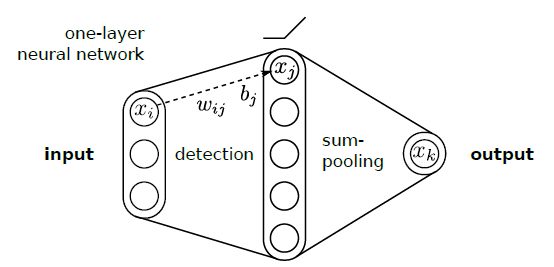
\includegraphics[width=10cm, height=5cm]{figures/one_layer_network}
	\label{fig:OneLayerNetwork}
\end{figure}

\begin{itemize}
\item $x_j = max(0, \sum_i x_i w_{ij} + b_j)$ (ReLU nonlinearity)
\item $x_k = \sum_j x_j$ (Sum pooling)
\end{itemize}

\end{frame}

% -------------------------------------------------------------------------------------------------
\begin{frame}{Example (2/2)}

$R_k$ of output layer: Total relevance that must be backpropagated:
\begin{itemize}
\item $R_k = x_k = \sum_j x_j$ 
\end{itemize}

$R_j$ of hidden layer: Taylor decomposition on $\{ \tilde{x}_j \} = 0$:
\begin{itemize}
\item $R_j = \frac{\partial R_k}{\partial x_j} \biggr\rvert_{\{ \tilde{x}_j \}} \cdot (x_j - \tilde{x}_j) = x_j = max(0, \sum_i x_i w_{ij} + b_j)$ 
\end{itemize}

$R_i$ of input layer: 
\begin{itemize}
\item $R_i = \sum_j \frac{\partial R_j}{\partial x_i} \biggr\rvert_{\{ \tilde{x}_i \}^{(j)}} \cdot (x_i - \tilde{x}_i^{(j)})$
\item $R_i = \sum_j \frac{w_{ij}^2}{\sum_{i'} w_{i'j}^2} R_j$ 
\end{itemize}

\end{frame}

%%%%%%%%%%%%%%%%%%%%%%%%%%%%%%%%%%%%%%%%%%%%%%%%%%%%%%%%%%%%%%%%%%%%%%%%%%%%%%%%%%%%%%%%%%%%%%%%%%%%
%%%%%%%%%%%%%%%%%%%%%%%%%%%%%%%%%%%%%%%%%%%%%%%%%%%%%%%%%%%%%%%%%%%%%%%%%%%%%%%%%%%%%%%%%%%%%%%%%%%%
%%%%%%%%%%%%%%%%%%%%%%%%%%%%%%%%%%%%%%%%%%%%%%%%%%%%%%%%%%%%%%%%%%%%%%%%%%%%%%%%%%%%%%%%%%%%%%%%%%%%
\section{Task description}

\begin{frame}{Task}

The task contains two parts
\begin{enumerate}
\item Numerical task
	\begin{itemize}
		\item Use the equations above to compute numerically the relevance of all layers of the network depicted in figure \ref{fig:OneLayerNetwork}.
		\item Use your own weight values ($w_{ij}$), but think on weighting schemes that are typically used in neural networks.
		\item Verify that the conservation and positivity rules properties apply.
		\item Provide descriptions of the interpretations
	\end{itemize}
\item Programmatic task
	\begin{itemize}
		\item Install, run.
		\item Change the number of training steps and see how the computed relevance changes.
		\item Provide descriptions of the interpretations of the relevance images with respect to the input images.
	\end{itemize}
\end{enumerate}

\end{frame}

%%%%%%%%%%%%%%%%%%%%%%%%%%%%%%%%%%%%%%%%%%%%%%%%%%%%%%%%%%%%%%%%%%%%%%%%%%%%%%%%%%%%%%%%%%%%%%%%%%%%
%%%%%%%%%%%%%%%%%%%%%%%%%%%%%%%%%%%%%%%%%%%%%%%%%%%%%%%%%%%%%%%%%%%%%%%%%%%%%%%%%%%%%%%%%%%%%%%%%%%%
%%%%%%%%%%%%%%%%%%%%%%%%%%%%%%%%%%%%%%%%%%%%%%%%%%%%%%%%%%%%%%%%%%%%%%%%%%%%%%%%%%%%%%%%%%%%%%%%%%%%
\begin{frame}{Literature}

\begin{itemize}
	\item 
\end{itemize}

\end{frame}

\end{document}